\begin{figure}
  \centering
  \footnotesize
  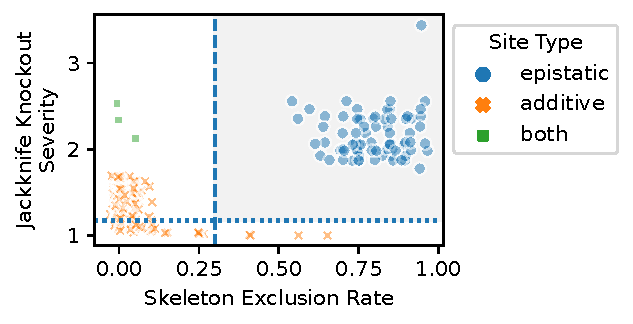
\includegraphics[width=\linewidth]{binder/teeplots/hue=site-type+style=site-type+viz=scatterplot-rect+x=skeleton-exclusion-rate+y=jackknife-knockout-severity+ext=}
  \vspace{-0.25in}
  \caption{%
    Use of knockout effect sizes and inclusion rates within ``skeletonized'' minimal viable genomes to distinguish between small-effect and epistatic genome sites.
  }
  \label{fig:epistatic}
  \vspace{-0.25in}
\end{figure}
